\section{N-BRWs WITH LIGHT TAILS}\label{sec:light_tails}

In \cite{exp_tails} Bérard and Gouéré studied the $N$-BRW whose point process is given by two independent draws from a distribution $p$ that has finite moment generating function in some neighbourhood of zero and whose spine can be centred (see \ref{eqn:t*exists}). In this section we adapt their results to the more general case of $N$-Branching Random Walks with finite logarithmic moment generating function in a neighbourhood of zero whose spine can be centered. Loosely speaking we extend their results to the case where the number of offspring are random and their position not necessarily independent of each other. We use the methods of \cite{exp_tails} for most proofs, adding details and adapting the arguments as necessary. \\

The inspiration to extend Bérard and Gouéré's result came from inspecting \cite{gantert2008asymptotics}, the article their analysis crucially relies on. I noticed that - presumably for simplicity - Bérard and Gouéré didn't use \cite{gantert2008asymptotics}'s results in their full generality. In \cite{mallein2018n} Mallein had a similar idea, however he went further: \cite{gantert2008asymptotics} heavily relies on \cite{mogul1975small} - the seminal paper of Mogulskii where he studies probabilities on the path-space of random walks. Mogulskii's results are valid for step distributions that are more general than the ones considered in \cite{gantert2008asymptotics} and thus Mallein extended the results of \cite{gantert2008asymptotics} and then applied this generalisation to obtain an even further generalisation of \cite{exp_tails} (see Section \ref{subsec:alpha_stable_spine} for a brief summary). The contribution of this section is hopefully to provide a slightly more satisfying and readable account than \cite{exp_tails}, while avoiding the highly technical machinery required by Mallein. To this end I have included many diagrams and tried to provide all the details required to easily follow the proofs. 

\subsection{The model}\label{subsec:The_model}
Consider the BRW $(\widehat{\bb{T}}, \widehat{V})$ governed by the point process $\widehat{\scr{L}}$ with logarithmic moment generating function $\widehat{\psi}$. Assume that (\ref{eqn:TreeAssumptions}), (\ref{eqn:t*exists}), (\ref{ass:killed_assumption_Lp}) and (\ref{ass:DacyingTails}) holds. Let $(\widehat{X}_n)_{n \geq 0}$ be the corresponding $N$-BRW and write $\max \widehat{X}_n$ and $\min \widehat{X}_n$ for the position of the right- and leftmost particle of $\widehat{X}_n$. We will show that 
\begin{equation}\nonumber
\hat{v}_N \defeq \lim_{n \to \infty} n^{-1}\max\widehat{X}_n = \lim_{n \to \infty} n^{-1}\min\widehat{X}_n
\end{equation} 
exists in $L^1$ and almost surely. The main result in this section is the analogue of Theorem 1 of \cite{exp_tails}: 
\begin{theorem}\label{thm:ExpTails_BrunDer_non_transformed}
As $N$ goes to infinity, 
\begin{equation}\nonumber
\widehat{v}_N = \widehat{\psi}'(t^*) - \frac{\pi^2 t^* \widehat{\psi}''(t^*)}{2 (\log N)^2} + o((\log N)^{-2}). 
\end{equation}
\end{theorem}


% Notice that if instead of $\widehat{\scr{L}}$ we used the point process $\widehat{\scr{L}}_N$ defined as $\widehat{\scr{L}}_N \defeq \sum^{N \land \# \scr{L}}_{i=1} \delta_{\scr{L}(i)}$ the resulting $N$-BRW would be exactly the same. Since $\# \widehat{\scr{L}}_N \leq N$ almost surely we see that assumption (\ref{ass:killed_assumption_Lp}) can be taken for granted. 


It will be more convenient to work with the BRW that is obtained after the transformation (\ref{eqn:transformation}). The resulting BRW will be denoted by $(\bb{T}, V)$ with point process $\scr{L}$ and logarithmic moment generating function $\psi$ that satisfies (\ref{eqn:BRW_V_Ass}). Observe that the associated random walk $(S_n)_{n \geq 0}$ with step distribution $X$ satisfies $\E X = 0$. Let $(X_n)_{n \geq 0}$ denote the $N$-BRW with point process $\scr{L}$ and take $X_0 \in \frak{M}_N$ deterministic. Assuming they exists, $v_N \defeq \lim_{n \to \infty} n^{-1} \max X_n$ is related to $\hat{v}_N$ by 
\begin{equation}\label{eqn:speed_relation}
v_N + \widehat{\psi}(t^*)= \hat{v}_N t^*, 
\end{equation}
as can be seen from (\ref{eqn:transformation2}). Therefore, what we will prove the following:
\begin{theorem}[Brunet-Derrida behaviour, centred form] \label{thm:ExpTails_BrunDer}
As $N$ goes to infinity, 
\begin{equation}\nonumber
v_N = - \frac{\pi^2 (t^*)^2 \widehat{\psi}''(t^*)} {2 (\log N)^2} + o((\log N)^{-2}). 
\end{equation}
\end{theorem}

\subsection{Properties of the model}
Clearly for all $t\in\R$ and $j \in [N], k \geq 1$ we have 
\begin{equation}\label{eqn:ExpTailsMaxIntegrable}
0 \leq e^{t\, \scr{L}_{n,j}(k)} \leq \sum_{|x|=1} e^{t\, V(x)}
\end{equation} so by assumption (\ref{ass:DacyingTails}) the $\scr{L}_{n,j}(k)$ have finite moment generating function in a neighbourhood of zero which implies exponentially decaying tails. It follows by Lemma \ref{lem:ExpTailsMax} that $\min X_n$ and $\max X_n$ are integrable and hence finite almost surely. Let $d(X_n) \defeq \max X_n - \min X_n$ be the diameter of $X_n$. The following result is analogous to Corollary 1 of \cite{exp_tails} and says that the diameter doesn't get too large:

\begin{proposition}\label{prop:diameter}
For any $N \geq 1$ and initial population $X_0 \in \frak{M}_N$, we have 
\begin{equation}\nonumber
\frac{d(X_n)}{n} \xrightarrow[n \to \infty]{a.s.,\, L^1} 0. 
\end{equation}
\end{proposition}

\begin{remark}
In \cite{mallein2018n} Mallein shows something stronger: he shows that there exists $C > 0$ such that for all $N$, 
\begin{equation}\nonumber
\Pr{d(X_n) > y} \leq C \left( \frac{N(\log N + \log y)}{y}\right)^2
\end{equation}
for all sufficiently large $n$. Using this we can get an upper bound on $\E\, d(X_n)$:
\begin{align*}
\E\, d(X_n) = \int\limits_0^\infty \Pr{d(X_n) > x} dx &\leq 1 + C N^3 \int\limits^\infty_N \left[\frac{\log x}{x}\right]^2 dx \\
													  &= 1 + C N^2[ \log^2 N + 2 \log N + 2]. 
\end{align*}
\end{remark}


% \begin{wrapfigure}{R}{0.5\textwidth}
% \centering
% 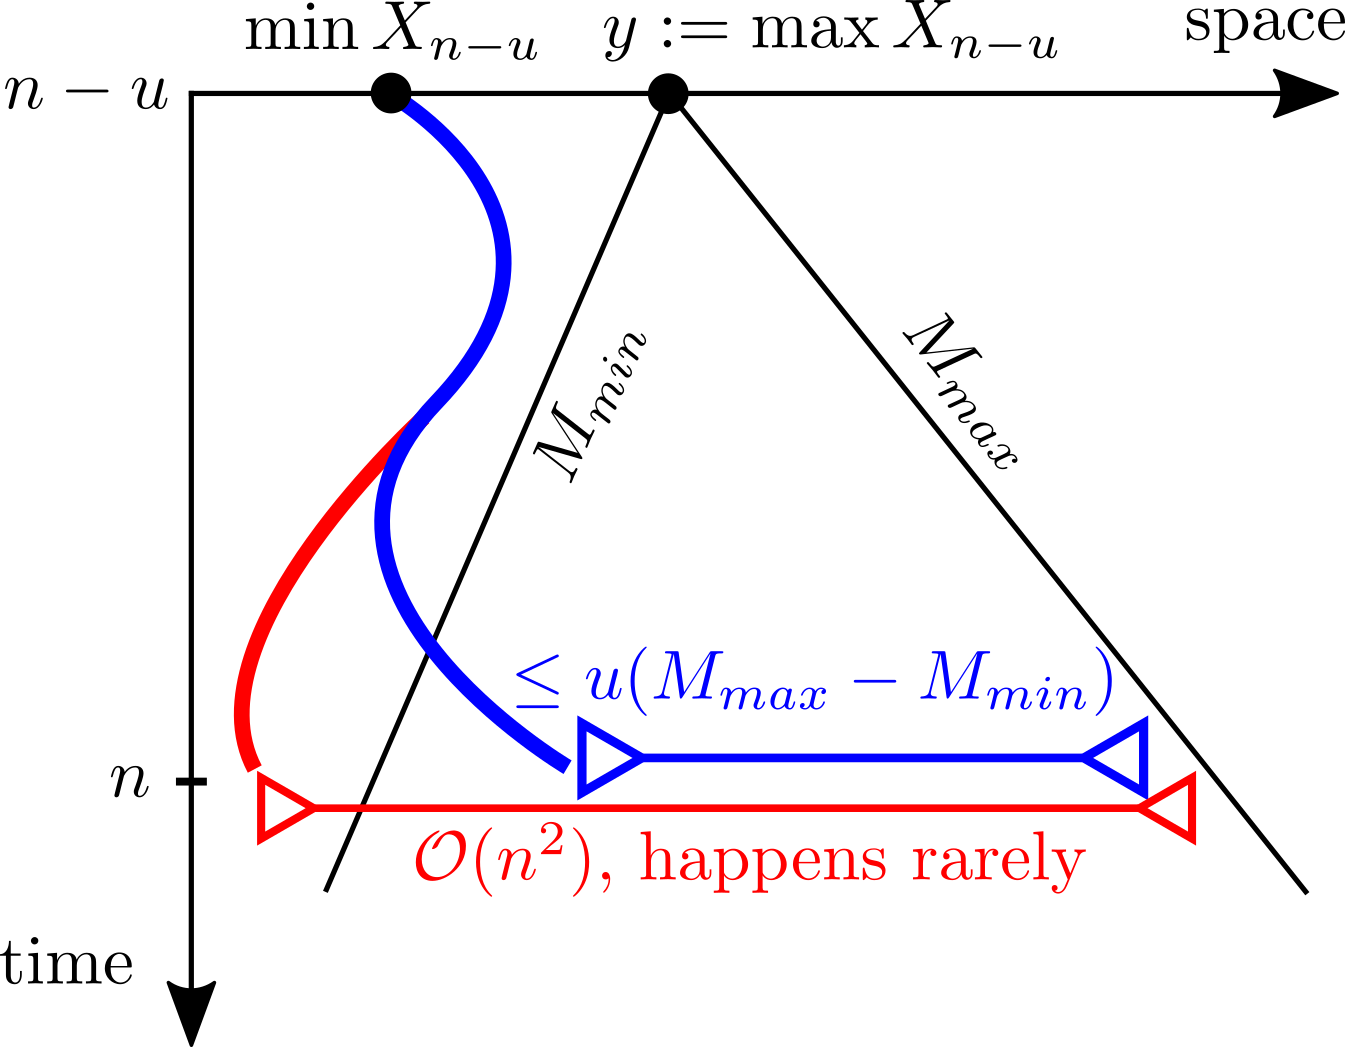
\includegraphics[width=0.45\textwidth]{graphics/g2.png}
% % \caption{\label{fig:frog1}This is a figure caption.}
% \end{wrapfigure}

\begin{proof}[Proof of Proposition \ref{prop:diameter}]
Let $u \in \N_+$ and for $n \geq u$ consider the process $X$ in the timeframe $\bbracket{n - u, n}$. Define 
\begin{align*}
M_{min} &\defeq \min\{ \scr{L}_{i, j}(N) \mid\, i \in \bbracket{n-u, n-1},\, j \in [N]\} \\
M_{max} &\defeq \max\{ \scr{L}_{i, j}(1) = \max\scr{L}_{i,j} \mid\, i \in \bbracket{n-u, n-1},\, j \in [N]\}
\end{align*} 
to be the smallest respectively largest random walk steps made between times $n-u$ and $n$. By Lemma \ref{lem:ExpTailsMax} both $M_{min}$ and $M_{max}$ are integrable. Write $y \defeq \max X_{n - u}$ for the rightmost particle's position at time $n-u$. \\

\begin{figure}[!h]
\centering
\begin{minipage}{0.45\textwidth}
  \centering
  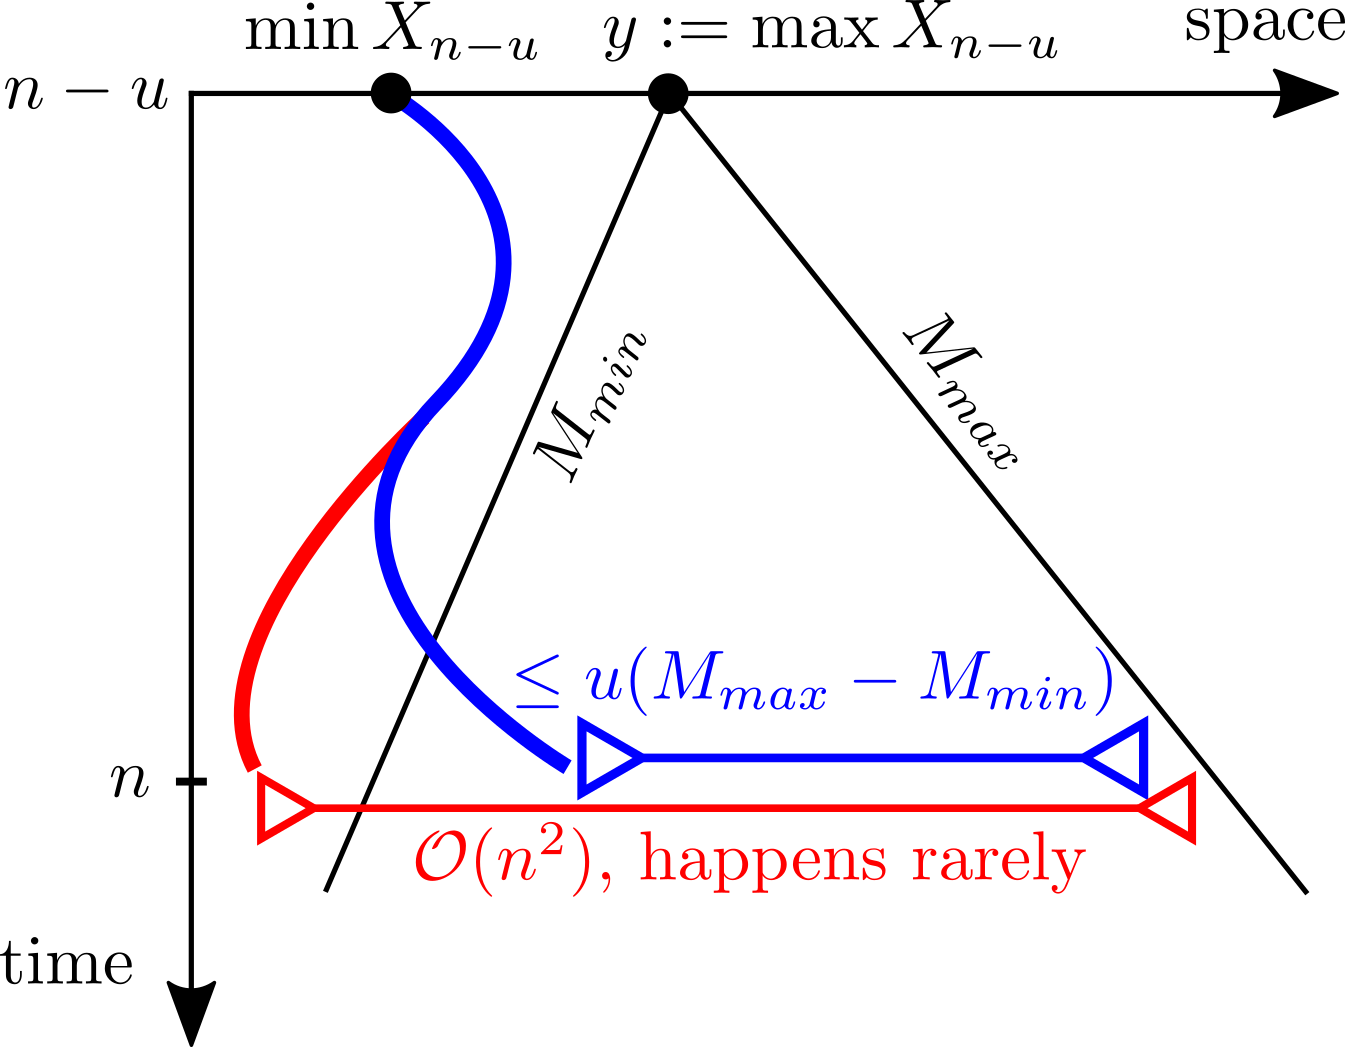
\includegraphics[width=\linewidth]{graphics/g2}
  \caption{Proof of Proposition \ref{prop:diameter}. }
  \label{fig:diam_proof}
\end{minipage}\hfill%
\begin{minipage}{0.45\textwidth}
  \centering
  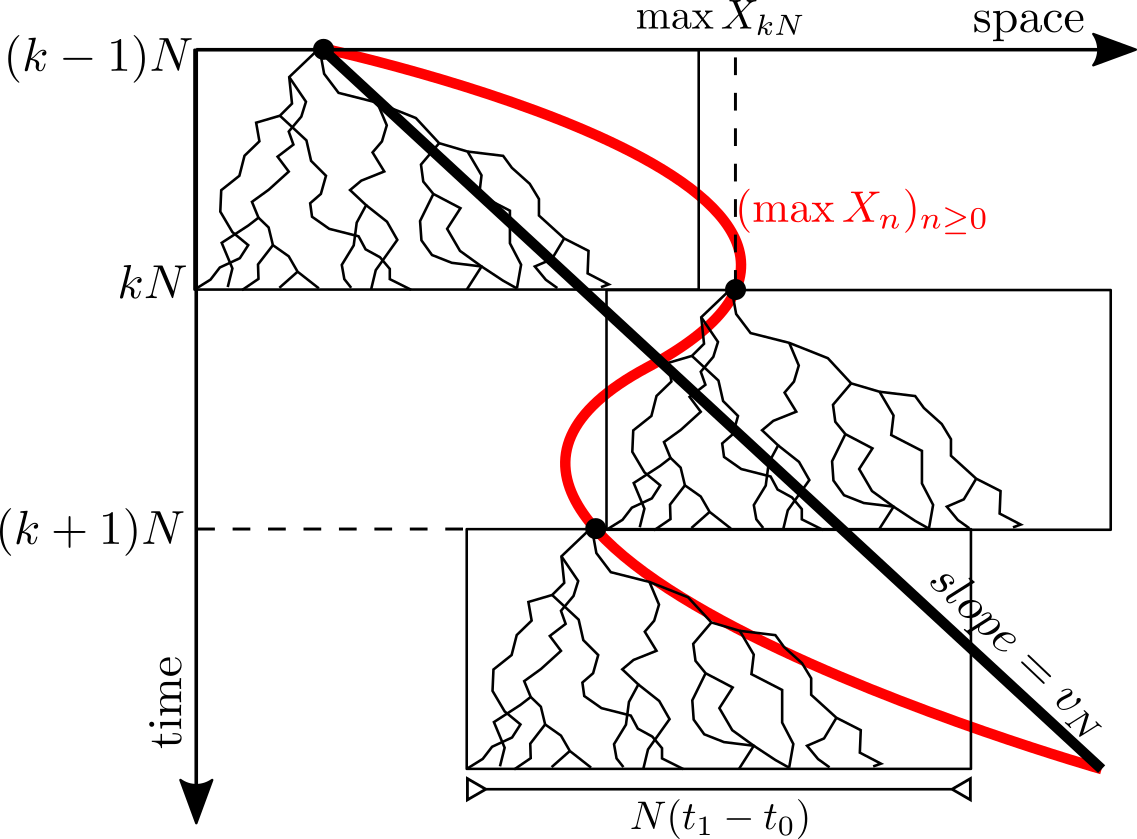
\includegraphics[width=\linewidth]{graphics/g1}
  \caption{Alternative proof of Proposition \ref{prop:diameter}. }
  \label{fig:diam_alternative_proof}
\end{minipage}
\end{figure}

Suppose that for each $k \in [u]$ we have $\min X_{n - u + k} < y + k m$. As all steps during branching are $ \geq M_{min}$, this implies in particular that the descendants of the particle at space-time point $(y, n-u)$ survive all selection steps until time $n$. Consider a Galton-Watson process $G \defeq (G_n)_{n \geq 0}$ with offspring distribution $\scr{L}$ coupled with the descendants of $(y, n-u)$ and consider the event $A_u \defeq \{ G_u > N\}$. Since $\Ex{\#\scr{L}} > 1$ and $\#\scr{L} \geq 1$ almost surely, $\Pr{A_u} \to 1$ as $u \uparrow \infty$ where $\Pr{A_u}$ is independent of $n$. Since at most $N$ descendants of $y$ can be alive at any time, on $A_u$ we must have $\min X_{n - u + k} \geq y + k_0 M_{min}$ for some $k_0$. By the definition of $M_{min}$ this must also hold for all $k \in \bbracket{k_0, u}$, in particular for $k = u$. Noting that $\max X_n \leq y + u M_{max}$, it follows that 
\begin{equation}\label{eqn:ExpTailDiamUpperBound}
d(X_n)\Ind_{A_u} \leq u (M_{max} - M_{min}), 
\end{equation}
with probability one. Fix $\epsilon > 0$ and take $u$ large enough so that $\Pr{A_u^c} < \epsilon^2$ and consider the decomposition
\begin{equation}\label{eqn:ExpTailsDiamDecomp}
\frac{d(X_n)}{n} = \frac{d(X_n)}{n} \Ind_{A_u} + \frac{d(X_n)}{n} \Ind_{A_u^c}. 
\end{equation}
The reader is referred to Figure \ref{fig:diam_proof} to help understanding. Taking expectations and then taking $n$ to infinity, the first term vanishes by (\ref{eqn:ExpTailDiamUpperBound}). The second term is upper bounded by $(\Pr{A_u^c} \Ex{d(X_n)^2 / n^2})^{1/2}$ using Hölder's inequality. A rough bound on $d(X_n)$ suffices: $d(X_n)$ is stochastically dominated by the sum of $n$ i.i.d. copies of $\max_{j \in [N]} \scr{L}_{0, j}(1) - \min_{j \in [N]} \scr{L}_{0,j}(N)$. Since the $\scr{L}_{n,j}(k)$ have exponentially decaying tails, by Lemma \ref{lem:ExpTailsMax} this yields $\Ex{d(X_n)^2} = \cal{O}(n^2)$ which implies that the second term in \ref{eqn:ExpTailsDiamDecomp} is $\cal{O}(\epsilon)$. Taking $\epsilon$ to zero concludes the proof of $L^1$ convergence. Almost sure convergence is a consequence of the proof of the next Proposition. 
\end{proof}

The original proof of Bérard and Gouéré is identical to ours up to the point where we consider the Galton Watson process $G$. Since they only considered binary BRWs, for $u > \log_2 N$ it is clear that $\Pr{A_u} = 1$ so that there is no need to decompose, they just conclude $d(X_n) \leq u(M_{max} - M_{min})$ almost surely. 

\begin{proposition}[{{\cite[Proposition 2]{exp_tails}}}]\label{prop:ExpTailsSpeedExistence}
There exists $v_N \in \R$ such that for any initial population $X_0 \in \frak{M}_N$ the following holds almost surely and in $L^1$:
\begin{equation}\nonumber
\lim\limits_{n \to \infty} \frac{\min X_n}{n} = \lim\limits_{n \to \infty} \frac{\max X_n}{n} = v_N. 
\end{equation}
\end{proposition}

\begin{proof}
First we treat the case $X_0 = N \delta_0$. Recall the definition of $(\scr{L}_{n, j})_{n \geq 0, j \in [N]}$ from the construction of $(X_n)_{n \geq 0}$. For each $r \geq 0$ we define the process $(X^r_n)_{n \geq 0}$ by shifting the origin of time by $r$. More precisely, $X^r_0 = N \delta_0$ for each $r \geq 0$ and given the process up to time $n \geq 0$, $X^r_{n+1}$ is be given by the $N$ rightmost particles of 
\begin{equation}\nonumber
\sum_{j = 1}^N \sum_{l \in \scr{L}_{r + n, j}} \delta_{X^r_n(j) + l}. 
\end{equation}
In other words, $(X^r_n)_{n \geq 0}$ is the $N$-BRW started from $N \delta_0$ constructed using $\scr{L}_{n \geq r, j \in [N]}$. Notice that $(X^r_n)_{n \geq 0}$ are identically distributed for each $r \geq 0$ and in particular, $(X^0_n)_{n \geq 0} = (X_n)_{n \geq 0}$ almost surely. From Lemma \ref{lem:monotonicity} it follows that 
\begin{equation}\label{eqn:subadd}
\max X^0_{n + m} \leq \max X^0_n + \max X^n_m \qquad \forall\, n,m \geq 0. 
\end{equation}
To see this consider running the process $(X^0_k)_{k \geq 0}$ up to time $n$, at which point we move all particles to the position of the rightmost particle at $\max X^0_n$ and continue running the process from this point for $m$ more steps. If we define $Z_{i,j} = \max X^i_{j - i}$ for $0 \leq i \leq j$ then (\ref{eqn:subadd}) reads $Z_{0, j} \leq Z_{0,i} + Z_{i,j}$ for all $0 \leq i \leq j$, which is familiar territory for Kingman's Subadditive Ergodic Theorem. We postpone showing that the conditions of the theorem hold to Lemma \ref{lem:ExpTailsKingmanHolds}. Applying Kingman's Subadditive Theorem yields 
\begin{equation}\nonumber
\lim_{n \to \infty} n^{-1} \max X_n = \lim_{n \to \infty} \Ex{n^{-1} \max X_n} = \inf_n \Ex{n^{-1} \max X_n} = v_N \in \R
\end{equation}
where the first limit is almost sure. Noting that the process $(-X_n)_{n \geq 0}$ also satisfies the hypothesis of the theorem, we can deduce from the identity $\min X_n = - \max (-X_n)$ that 
\begin{equation}\nonumber
\lim_{n \to \infty} n^{-1} \min X_n = \lim_{n \to \infty} \Ex{n^{-1} \min X_n} = \inf_n \Ex{n^{-1} \min X_n} = \tilde{v}_N \in \R
\end{equation}
exists too, where the first limit is almost sure. From Proposition \ref{prop:diameter} we immediately get $\tilde{v}_N = v_N$ by uniqueness of $L^1$ limits, which also yields almost sure convergence in Proposition \ref{prop:diameter}. The proof is thus complete in the case $X_0 = N \delta_0$. By translation invariance of the dynamics of the system the result also follows for initial states of the form $N \delta_{x_0}$ for any $x_0 \in \R$. Finally, for arbitrary $X_0 \in \frak{M}_N$ note that the result is a consequence of Lemma \ref{lem:monotonicity} and a sandwiching argument between the initial states $N \delta_{\min X_0}$ and $N \delta_{\max X_0}$. 
\end{proof}

% \begin{wrapfigure}{R}{0.5\textwidth}
% \centering
% 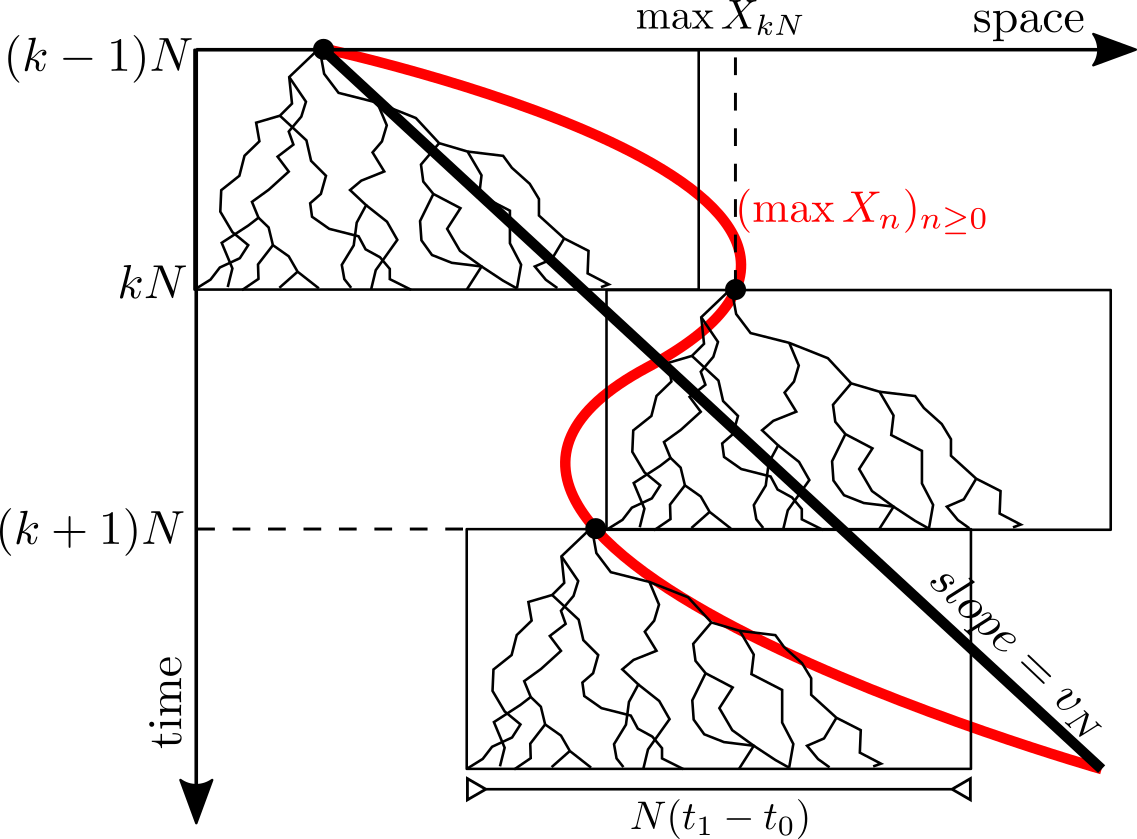
\includegraphics[width=0.45\textwidth]{graphics/g1.png}
% % \caption{\label{fig:frog1}This is a figure caption.}
% \end{wrapfigure}

Inspecting the previous proof, we see that the existence of $v_N$ and $\tilde{v}_N$ (the almost sure and $L^1$ limits of the left- and rightmost particles) when started from $X_0 = N \delta_0$ was shown without relying on Proposition \ref{prop:diameter}. Therefore it might be possible to go the other way: if we can show that $v_N = \tilde{v}_N$ then we can \textit{deduce} Proposition \ref{prop:diameter} from Proposition \ref{prop:ExpTailsSpeedExistence}. We do so by an argument inspired by one of Prof. Berestycki's suggestions:

\begin{proof}[Alternative proof of Proposition \ref{prop:diameter}]
Consider $(X_n)_{n \geq 0}$ over the timeframe $\bbracket{0, N}$. Let $Y \defeq (Y_n)_{0 \leq n \leq N}$ be a branching random walk (without selection) driven by $\scr{L}$ that is coupled with $(X_n)_{0 \leq n \leq N}$ as follows. Start $(Y_n)_{0 \leq n \leq N}$ from a single particle at zero and couple it with the descendants of $\max X_0$ independently of the rest of $(X_n)_{0 \leq n \leq N}$. Define $M^Y_{min}, M^X_{min}$ and $M^Y_{max}, M^X_{max}$ to be the minimum and maximum of all steps taken by $Y$ and $X$ up to time $N$. Finally, let $M_{min} \defeq M^X_{min} \land M^Y_{min}$ and $M_{max} \defeq M^X_{max} \lor M^Y_{max}$. Since $\Ex{\# \scr{L}} > 1$, the probability $\rho_1$ that the number of particles in $Y$ has reached $N$ by time $N$ is strictly positive. By Lemma \ref{lem:ExpTailsMax} $M_{max}, M_{min}$ are finite, so one can certainly find $C > 0$ such that $\rho_2 \defeq \PrCond{-C \leq M_{min} \leq M_{max} \leq C }{\# Y_N \geq N} > 0$. We are interested in the event
\begin{equation}\nonumber
E_Y \defeq \{ \# Y_N \geq N \} \cap \{-C \leq M_{min} \leq M_{max} \leq C \}. 
\end{equation}
The probability of $E_Y$ can be expressed in terms of $\rho_1$ and $\rho_2$:
\begin{equation}\nonumber
\Pr{E_Y} \\
= \Pr{\# Y_N \geq N} \PrCond{-C \leq M_{min} \leq M_{max} \leq C }{\# Y_N \geq N} \geq \rho_1 \rho_2 > 0.
\end{equation}
Now in an analogous way we can place copies of $Y$ denoted by $((Y^{(k)}_n)_{0 \leq n \leq N})_{k \geq 0}$ at the space-time points $(\max X_{kN}, kN)_{k \geq 0}$. By the second Borel-Cantelli lemma it follows that almost surely infinitely many of the corresponding events $E_{Y^{(k)}}$ must occur. This in turn implies that for infinitely many $k \geq 0$ the diameter is less than $2NC$ for some time $n \in [Nk, N(k+1))$. This immediately yields $\tilde{v}_N = v_N$ and completes the proof. 
\end{proof}

\begin{proposition}[{{\cite[analogue of Proposition 3]{exp_tails}}}]\label{prop:increasing_speed}
The sequence $(v_N)_{N \geq 1}$ is non-decreasing. 
\end{proposition}
\begin{proof}
This is again a consequence of Lemma \ref{lem:monotonicity}. 
\end{proof}




\subsection{Brunet-Derrida behaviour}\label{sec:ExpTails_BrunDer}
From here on in this essay, unless specified otherwise, all $N$-BRWs are started from $N\delta_0$ and all BRWs are started from $\delta_0$. We can do this without loss of generality thanks to Proposition \ref{prop:diameter}. First let us describe the coupling between the $N$-BRW and $N$ independent BRWs which allows us to apply Theorems \ref{thm:infty_good} and \ref{thm:finite_good} to our study of $N$-BRWs. Let $(\text{BRW}_j)_{j \in [N]} = ((\bb{T}_j, V_j))_{j \in [N]}$ be $N$ independent copies of the BRW with point process $\scr{L}$. Define $\scr{T}_n \defeq \bigsqcup_{j=1}^N \{ x \in \bb{T}_j \,:\, |x|=n \}$ to be the disjoint union of vertices at depth $n$. We now inductively define a sequence $(G_n)_{n \geq 0}$ of random subsets of $\scr{T}_n$, each with exactly $N$ elements. These random subsets will correspond to the particles alive in the coupled $N$-branching random walk at time $n$. Define $G_0 = \scr{T}_0$ and given $G_n$, define $H_n$ to be the vertices in $\scr{T}_{n+1}$ that descend from vertices in $G_n$. Finally, set $G_{n+1}$ to be the set of $N$ vertices in $H_n$ with the greatest value. If we now define (with some abuse of notation) $\frak{X}_n = \sum_{u,j : u \in G_n \cap \bb{T}_j} \delta_{V_j(u)}$ then $(\frak{X}_n)_{n \geq 0}$ has the same distribution as $(X_n)_{n \geq 0}$ started from $N \delta_0$. 

\subsubsection{Upper bound}\label{subsec:upper_bound}
\begin{proof}[Proof of upper bound in Theorem \ref{thm:ExpTails_BrunDer}]
As mentioned before, we treat the case $X_0 = N \delta_0$. For notational simplicity define $\chi = \pi^2 (t^*)^2 \widehat{\psi}''(t^*) / 2$. Our aim is to show $v_N \defeq \lim_{n \to \infty} \Ex{n^{-1} \max X_n} \leq -  \chi / (\log N)^2 + o((\log N)^{-2})$. Recalling the proof of Proposition \ref{prop:ExpTailsSpeedExistence}, we know by subadditivity that
\begin{equation}\label{eqn:ExpTailsSubaddDecomp1}
v_N \leq \frac{\Ex{\max X_n}}{n} \qquad\qquad\forall\, n \in \N. 
\end{equation}
In light of the desired correction term, we decompose (\ref{eqn:ExpTailsSubaddDecomp1}) into
\begin{equation}\nonumber
\Ex{\max X_n} \leq - \frac{\chi}{(\log N)^2} + \Ex{\max X_n \Ind_{\{\max X_n \geq -n \chi (\log N)^{-2} \}}}. 
\end{equation}
However, this is not the exact form of the RHS that we will work with. Let $\gamma \in (0,1)$ and $\epsilon = \epsilon(N)$ whose precise form we will choose later, but will be approximately $\chi (\log N)^{-2}$ as $N \to \infty$. We go on to show that in
\begin{equation}\nonumber
\Ex{\frac{\max X_n}{n}} \leq  - (1 - \gamma)\epsilon + \Ex{\frac{\max X_n}{n} \Ind_{\{\max X_n \geq  -n (1 - \gamma) \epsilon \}}}
\end{equation}
the last term is $o((\log N)^{-2})$. This will yield the desired upper bound on $v_N$ if we take $\gamma \to 0$. We further decompose the problem: for $\delta > 0$ we have
\begin{align*} 
\E \bigg[\frac{\max X_n}{n} &\Ind_{\{\max X_n \geq - n (1 - \gamma)\epsilon \}}\bigg] \leq \\
							&\delta\underbrace{\Pr{\frac{\max X_n}{n} \geq -(1 - \gamma)\epsilon }}_{\circled{1}} + \underbrace{\Ex{\frac{\max X_n}{n} \Ind_{\{ \delta n \leq \max X_n \}}}}_{\circled{2}}. 
\end{align*}
First we show that for an appropriate scaling of $\epsilon=\epsilon(N)$ and $n = n(N)$ we have $\circled{1} = o((\log N)^{-2})$. Set $n = \ceil{N^\xi}$ for some $0 < \xi < \gamma$ and $m = m(N) \leq n$ whose exact form we'll specify soon. Let $B$ be the number of vertices in $\sqcup_{i=0}^n G_i$ that are $(m, - \epsilon)$-good with respect to their corresponding BRWs. Let $u_0, u_1, ..., u_n$ be a path in $\bb{T}_{i_0}$ for some $i_0 \in [N]$ such that $u_0 = root_{i_0}$ and $u_n \in G_n$ with $V_{i_0}(u_n) = \max X_n$. In other words, let $BRW_{i_0}$ be the random walk that the rightmost particle of the coupled $N$-branching random walk lives in at time $n$, and let $u_0, ..., u_n$ be the path connecting it to the corresponding root. Define the event $E \defeq \{ \max X_n \geq - n (1 - \gamma)\epsilon \}$, and apply Lemma \ref{lem:ExpTailsGoodSequencesTechnical} to the sequence of real numbers $(V_{i_0}(u_i))_{i \in [n]}$. It follows that on $E$, for any $K > 0$, either one of the random walk steps along the path is $> K$ or $B \geq \frac{\gamma\epsilon}{K + \epsilon}\frac{n}{m} - \frac{K}{K + \epsilon} \eqdef B^\#(N, \gamma, K)$. This yields
\begin{equation}\label{eqn:ExpTailsEBound}
\circled{1} = \Pr{E} \leq \Pr{M \geq K} + \Pr{B \geq B^\#},  
\end{equation}
where $M \defeq \max \{\max \scr{L}_{l, j} \mid\, l \in \bbracket{0, n - 1},\, j \in [N]\}$. Set $\beta \in (0, \bb{V}(X))$ and let $\theta > 0$ be as in Theorem \ref{thm:finite_good}. Let $\lambda > 0$, and define 
\begin{equation}\nonumber
m \defeq \ceil*{ \left[\frac{2 \theta}{\pi^2}\right]^{3/2} \left( \frac{(1 + \lambda) \log N}{(\bb{V}(X) - \beta)^{1/2}}\right)^3},
\end{equation} 
and $\epsilon \defeq \theta\, m^{-2/3}$. $m$ is carefully chosen so that by Theorem \ref{thm:finite_good}, 
\begin{equation}\label{eqn:ExpTailsProof}
\rho(m, \epsilon) \leq N^{-(1 + \lambda)} 
\end{equation}
for all large $N$. Also let $K = \kappa \log N$ for $\kappa > 0$ and observe that $B^\# > 0$ for large enough $N$ independently of $\kappa$. Thus (\ref{eqn:ExpTailsEBound}) turns into
\begin{equation}\nonumber
\circled{1} = \Pr{E} \leq \underbrace{\Pr{M \geq K}}_{\circled{1a}} + \underbrace{\Pr{B \geq 1}}_{\circled{1b}}. 
\end{equation}

$\circled{1a}$: As noted before, $(\max \scr{L}_{i,j})_{i \geq 0, j \in [N]} = (\scr{L}_{i, j}(1))_{i \geq 0, j \in [N]}$ are i.i.d. with common distribution $\max \scr{L}$ and have exponentially decaying tails so that there exists $C, \phi, K_0 > 0$ such that for all $K > K_0$ it holds that $\Pr{\max \scr{L} > K} \leq C \exp(-\phi K)$. By a calculation similar to the proof of Lemma \ref{lem:ExpTailsMax}, for all large enough $\kappa$ we get
\begin{align*}
\Pr{M \geq K} &= 1 - (1 - \Pr{\max \scr{L} > K})^{Nn} \leq 1 - (1 - C \exp(-\phi K))^{Nn} \\
			  &= 1 - (1 - C N^{-\phi \kappa})^{Nn} \leq C N^{-\phi \kappa} Nn = C N^{1 + \xi - \phi \kappa}. 	
\end{align*} 
Thus, $\Pr{M \geq K} = o((\log N)^{-2})$ for $\kappa > 2/\phi$. \\

$\circled{1b}$: Consider a vertex $u \in \bb{T}_{j_0}$ for some $j_0 \in [N]$ with $|u| \leq n$. The event $\{u \in G_d\}$ is measurable with respect to the sigma algebra generated by the random variables $\{ V_j(v) \mid\, j \in [N],\, v \in \bb{T}_j,\, |v| \leq |u|\}$. On the other hand, the event $\{ u \text{ is }(m, - \epsilon) \text{-good}\}$ is determined by the variables $\{ V_{j_0}(v) - V_{j_0}(u) \mid\, v \in \bb{T}_{j_0},\, |u| < |v| \}$, so that the two events are independent. We can write $B$ as 
\begin{equation}\nonumber
B = \sum\limits_{i=1}^N \sum\limits_{u \in \bb{T}_i} \Ind_{\{u \text{ is } (m, - \epsilon)\text{-good}\}} \Ind_{\{u \in G_d \text{ for some d} \leq n \}}. 
\end{equation}
Taking expectations gives 
\begin{equation}\nonumber
\Ex{B} \leq N(n+1)\rho(m, \epsilon) = \cal{O}(N^{\xi -\lambda}) = o((\log N)^{-2}) \qquad\text{as $N$ goes to infinity}, 
\end{equation}
where we used that $G_n$ has $N$ elements for all $n$. Applying Markov's inequality to $B$ and combining with our estimate of $\circled{1a}$ gives $\circled{1} = o((\log N)^{-2})$ as desired. \\

We now turn to showing $\circled{2} = o((\log N)^{-2})$. Consider the obvious inequality $\exp(\max X_n) \leq \sum_{j \in [N]} \sum_{x \in \bb{T}_j : |x| = n} \exp(V_j(x))$. It follows from the Many-to-One lemma that 
\begin{align*}
\Ex{\exp(\max X_n)} \leq N\, \E\sum\limits_{|x| = n} \exp(V(x)) = N. 
\end{align*}
Now apply Lemma \ref{lem:ExpTailBound} with $x = \max X_n$ and $a = \delta n$ and take expectations to get 
\begin{align*}
\Ex{\max X_n \Ind_{\{\max X_n \geq \delta n \}}} &\leq \Ex{\exp(X_n - \delta n / 2)} \leq N \, e^{-\delta n / 2} = o((\log N)^{-2}).
\end{align*}
This concludes the proof of the upper bound: we have shown that for any choice of $\gamma \in (0,1)$, $\beta \in (0, \bb{V}(X))$ and $\lambda > \xi > 0$ we have
\begin{equation}\label{eqn:ExpTailResultTally}
v_N \leq \Ex{\ceil{N^\xi}^{-1} \max X_{\ceil{N^\xi}}} \leq - (1 - \gamma) \frac{\pi^2 (\bb{V}(X) - \beta)}{2 (1 + \lambda)^2(\log N)^2} + o((\log N)^{-2}). 
\end{equation}
Taking $\gamma, \beta, \lambda$ and $\xi$ to zero gives the desired result. 
\end{proof}

\begin{remark}
There are three notable differences between our and Bérard and Gouéré's proof of the upper bound. First, I restructured the material in a way to make the strategy of the proof clearer - something I found to be lacking in \cite{exp_tails}. Second, since they only consider binary BRWs, obtaining the bound on $\circled{1b}$ is easier, while we had to rely on Lemma \ref{lem:ExpTailsMax} which although looks classical, I couldn't find a reference for. Lastly, our proof of $\circled{2} = o((\log N)^{-2})$ is easier to follow. 
\end{remark}

Here is a summary of the variables used in the previous proof, collected in a table to ease understanding:
\begin{center}
\begin{tabular}{|c|c||c|c|} 
 \hline
 % Variable 	& Definition 			& Variable 	& Definition 								            \\
 $\gamma$ 	& $\in (0, 1)$ 			&	$\bb{V}(X)$		& $2 \chi / \pi^2$		        \\

 $\delta$ 	& $\in (0, \infty)$ 	&  	$\beta$			& $\in (0, \bb{V}(X))$								            \\ 

 $\xi$ 		& $\in (0, \gamma)$ 	&	$\theta$	& as in Theorem \ref{thm:finite_good}			                             \\ 

 $\kappa$	& $\in (0, \infty)$		&	$K$ 				& $\kappa \log N$	                 \\

$\chi$ 			& $\pi^2 (t^*)^2 \widehat{\psi}''(t^*) / 2$ &  $m$ & $\ceil*{ \left[\frac{2 \theta}{\pi^2}\right]^{3/2} \left( \frac{(1 + \lambda) \log N}{(\bb{V}(X) - \beta)^{1/2}}\right)^3}$\\

$\lambda$	& $\in (0, \infty)$ & $\epsilon$ & $\theta\,m^{-2/3}$ \\

$n$ 		& $\ceil{N^\xi}$     & & \\

 \hline
\end{tabular}
\end{center}










\subsubsection{Lower bound}\label{subsec:lower_bound}
\begin{proof}[Proof of lower bound in Theorem \ref{thm:ExpTails_BrunDer}]

Let $\lambda, \eta \in (0,1)$ and let 
\begin{equation}\nonumber
\epsilon \defeq \frac{\chi}{(1-\lambda)^2(\log N)^2}. 
\end{equation}
With this choice Theorem \ref{thm:infty_good} gives $\rho(\infty, - \epsilon) = N^{\lambda - 1 + o(1)}$ as $N \to \infty$. Recall now the construction of $(X^r_n)_{n, r \geq 0}$ using $(\scr{L}_{n, j})_{n \geq 0, j \in [N]}$ from the proof of Proposition \ref{prop:ExpTailsSpeedExistence}. Define the random variables $\Gamma_0 \defeq 0$ and $J_0 \defeq 0$ and set $i = 0$. Given $\Gamma_i$ and $J_i$ inductively define $L_{i+1} \defeq n \land \inf\{ k \mid\, \min X^{\Gamma_i}_k \geq -(1+\eta)\epsilon k\}$. Finally, let $\Gamma_{i+1} \defeq \Gamma_i + L_{i+1}$ and $J_{i+1} \defeq J_i + \min X^{\Gamma_i}_{L_{i+1}}$. See Figure \ref{fig:regen_structure} for the meaning of $J_i, L_i, \Gamma_i$. Using words, at each time $\Gamma_i$ we move all particles to the left-most particle's position $\min X_{\Gamma_i}$ and continue the process from there - giving us a lower bound on $(X_n)_{n \geq 0}$. By Lemma \ref{lem:monotonicity} it follows that 
\begin{equation}\label{eqn:regenTime}
\min X_{\Gamma_i} \geq J_i \qquad\forall\, i \geq 0. 
\end{equation}
Observe now that $\Gamma_{i+1} - \Gamma_i$ is an i.i.d. sequence with common distribution $L \defeq n \land \inf \{ k \mid \min X_k \geq - (1+\eta)\epsilon k\}$. Similarly, the sequence $J_{i+1} - J_i$ is also i.i.d. with common distribution $\min X_L$. The strong law of large numbers gives 
\begin{equation}\nonumber
\lim\limits_{i \to \infty} \frac{\min X_{\Gamma_i}}{i} = \lim\limits_{i \to \infty} \frac{\min X_{\Gamma_i}}{\Gamma_i} \frac{\Gamma_i}{i} = v_N \E L
\end{equation}
almost surely. However, by (\ref{eqn:regenTime}) we also have
\begin{equation}\nonumber
\liminf\limits_{i \to \infty} \frac{\min X_{\Gamma_i}}{i} \geq \liminf\limits_{i \to \infty} \frac{J_i}{i} = \Ex{\min X_L}.
\end{equation}
Denote $B \defeq \{ \min X_k < - (1+\eta)\epsilon \text{ for all } k \in [n]\}$ and define the random variable $\Theta_n$ to have the law of $\min \{\scr{L}_{i, j}(N) \mid\, j \in [N],\, 0 \leq i \leq n - 1 \}$. Combining the obvious inequalities $\min X_L \geq -(1 + \eta)\epsilon L \Ind_{B^c} + n \Theta_n \Ind_B$ and $1 \leq L \leq n$ with the above bounds we get
\begin{equation}\label{eqn:lowerBdd}
v_N \geq \frac{\Ex{\min X_L}}{\E L} \geq -(1+\eta)\epsilon (1 + n\Pr{B}) - n\Ex{|\Theta_n| \Ind_B}. 
\end{equation}
By Hölder's inequality $\Ex{|\Theta_n| \Ind_B} \leq \sqrt{\Ex{\Theta_n^2}\Pr{B}}$. By Lemma \ref{lem:ExpTailsMax} we know that $\Theta_n$ has exponentially decaying tails, so in particular is square-integrable. To prove the lower bound we only need a suitably strong upper bound on $\Pr{B}$. The remainder of the proof is dedicated to this. \\

\begin{figure}
\centering
\begin{minipage}{0.45\textwidth}
  \centering
  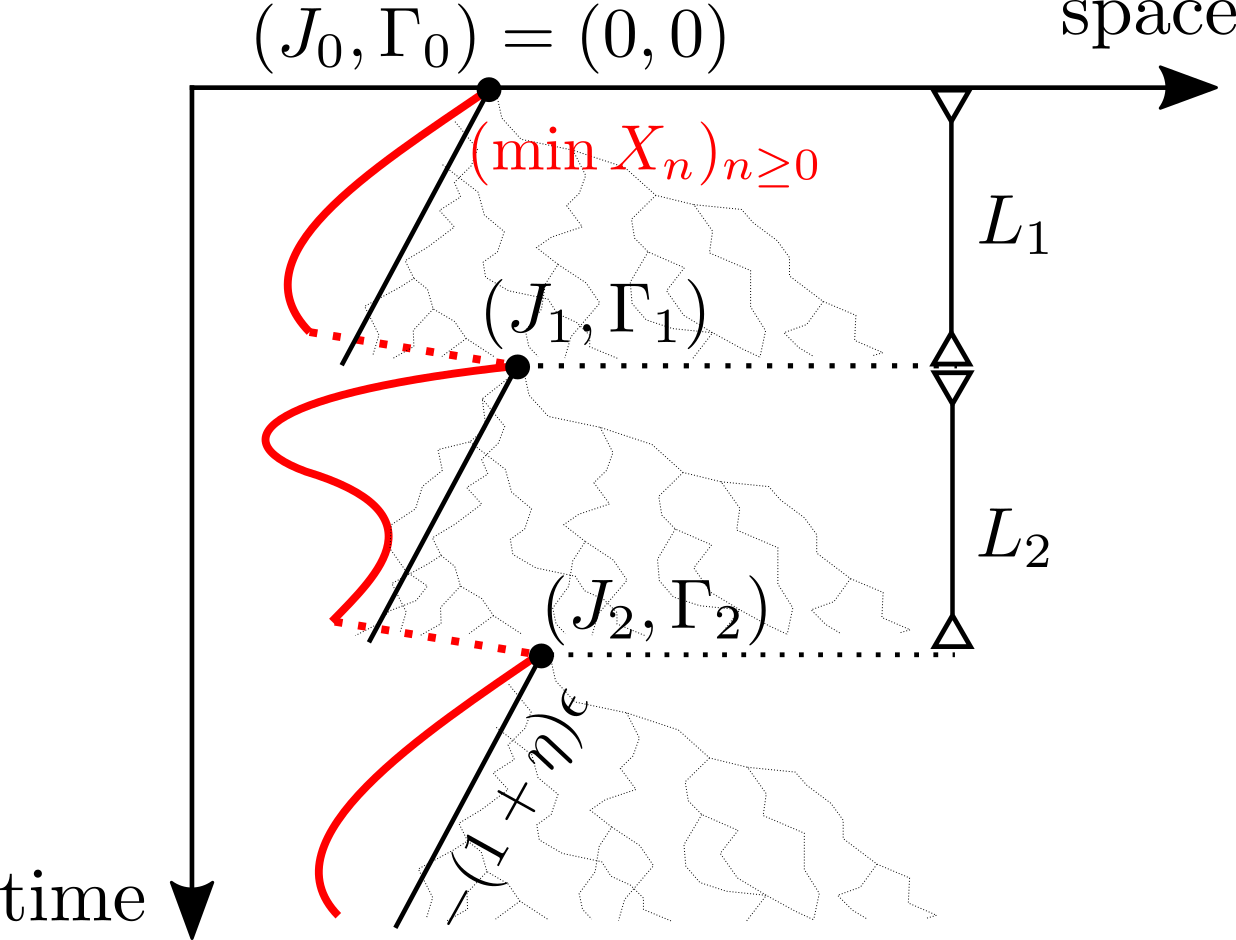
\includegraphics[width=\linewidth]{graphics/g4}
  \caption{The regeneration structure. }
  \label{fig:regen_structure}
\end{minipage}
\begin{minipage}{0.45\textwidth}
  \centering
  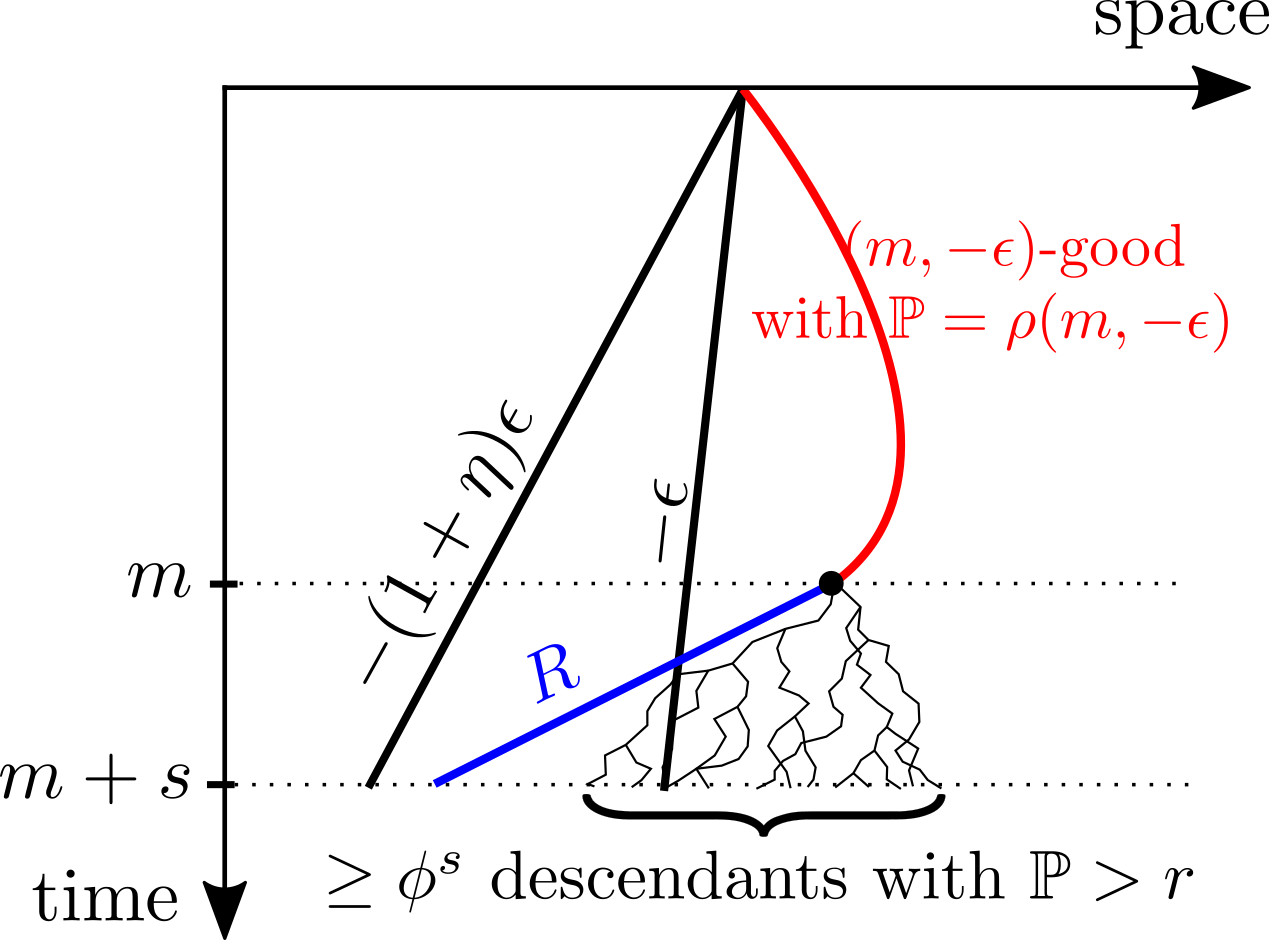
\includegraphics[width=\linewidth]{graphics/g3}
  \caption{The paths $(w_i)_{i \in [n]}$. }
  \label{fig:weird_constant_choice}
\end{minipage}\hfill%
\end{figure}


Since $1 < \Ex{\#\scr{L}} = \E[\sum_{|x|=1} 1]$, by the monotone convergence theorem we can take $R > 0$ such that $1 < \E\sum_{|x|=1} \Ind_{\{ V(x) \geq -R\}}$. If we let $(M_n)_{n \geq 0}$ be the Galton Watson process started from $M_0 = 1$ with offspring law $\sum_{|x|=1} \Ind_{\{ V(x) \geq -R\}}$ then by Lemma \ref{lem:ExpTailsGW} there exist $\phi > 1$ and $r > 0$ such that $\Pr{M_n \geq \phi^n} \geq r$ for all $n \geq 0$. Define now $s \defeq \ceil{\frac{\log N}{\log \phi}} + 1$ and $m \defeq \ceil{\frac{Rs}{\eta\, \epsilon}}$ and finally set $n = s + m$. Consider a vertex $u$ at depth $m$ in one of the $BRW_i$. The probability that there are at least $\phi^s$ distinct paths $u \eqdef u_m, ..., u_n$ with $V_i(u_{k+1}) - V_i(u_k) \geq R$ for all $k \in \bbracket{m, n - 1}$ is greater than $r$ by our previous discussion. Recall that the probability of the root being $(m, - \epsilon)$-good is $\rho(m, - \epsilon)$. We see that then the probability of observing a path $root = w_0, ..., w_n$ in $BRW_i$ such that $V_i(w_k) \geq - k \epsilon$ for $k \in [m]$ and $V_i(w_{k+1}) - V_i(w_k) \geq R$ for $k \in \bbracket{m, n-1}$ is at least $\rho(m, - \epsilon) r$. By the choice of $s$ and $m$, such a path must also be $(n,  - (1+\eta)\epsilon)$-good as shown on Figure \ref{fig:weird_constant_choice}. Indeed, given our choice of $\epsilon, \eta, R$ and $s$ and assuming the path $(w_i)_{i \in [n]}$ is $-\epsilon$-good up to time $m$, it is $(n, -(1+\eta)\epsilon)$-good if and only if for each $k \in [s]$ we have
\begin{equation}\nonumber
-m\epsilon - kR \geq -\epsilon(1 + \eta)(m + k) \quad\iff\quad m \geq \frac{k(R - \epsilon(1 + \eta))}{\eta \epsilon}
\end{equation}
which clearly holds true for $m \defeq \ceil{\frac{Rs}{\eta\, \epsilon}}$. \\

For $i \in [N]$ define $A_i$ to be the event that $BRW_i$ contains no more than $\phi^s$ distinct $(n, - (1+\eta)\epsilon)$-good paths starting at the root. By independence we get
\begin{equation}\nonumber
\Pr{\bigcap\limits_{i=1}^N A_i} \leq (1 - \rho(m, \epsilon) r)^N. 
\end{equation}
On the event $B \cap [\cap_{i=1}^N A_i]^c$ one of the $BRW_i$ has $> \phi^s > N$ particles at time $n$ that have stayed to the right of the space time line with slope $ - (1 + \eta)\epsilon$ until time $n$. By definition, on $B$ this implies that there are $> N$ particles alive in the $N$-branching random walk which is impossible. Therefore $B \cap [\cap_{i=1}^N A_i]^c = \varnothing$ and so $B \subset \cap_{i=1}^N A_i$. Using the fact that $\rho(m, - \epsilon) \leq \rho(\infty, - \epsilon) = N^{\lambda - 1 + o(1)}$ and the inequality $1 - x \leq \exp(-x)$ for all $x \in \R$, we get
\begin{equation}\label{eqn:ExpTailsBBound}
\Pr{B} \leq \Pr{\bigcap\limits_{i=1}^N A_i} \leq \exp(-N^{\lambda + o(1)})
\end{equation}
Combining the above estimate of $\Pr{B}$ with (\ref{eqn:lowerBdd}) results in 
\begin{equation}\nonumber
v_N \geq - \frac{\chi (1 + \eta)}{(1 - \lambda)^2(\log N)^2} + o((\log N)^{-2}). 
\end{equation} 
As $\lambda$ and $\eta$ can be taken arbitrarily small, the desired result follows. 
\end{proof}

\newpage
\subsection{Discussion}
This section is based in part on \cite{exp_tails} Section 8 and aims to give a non-rigorous picture of the main idea of the proof in Sections \ref{subsec:upper_bound} and \ref{subsec:lower_bound}. Fix some point process that satisfies the assumptions of Theorem \ref{thm:ExpTails_BrunDer_non_transformed} and let $v_N$ and $v$ be the asymptotic speeds of the corresponding $N$-BRW and $BRW$. Consider the coupling of $(BRW_j)_{j \in [N]}$ (N i.i.d. copies of the BRW) and $(X_n)_{n \geq 0}$ (the $N$-BRW) that was introduced at the beginning of Section \ref{sec:ExpTails_BrunDer}. The proof of the Brunet-Deridda behaviour hinged on the idea that under this coupling, heuristically speaking the following properties are equivalent:
\begin{enumerate}[(a)]
{\item \vspace{-1mm} $(BRW_j)_{j \in [N]}$ do not survive killing below the speed $v - \epsilon$
\item \vspace{-3mm} $v_N < v - \epsilon$. }
\end{enumerate}
\vspace{-3mm}
Intuitively this should be true: if (a) holds then we certainly can't expect the $N$-BRW to propagate faster than $v - \epsilon$ since it is dominated by $(BRW_j)_{j \in [N]}$ through the coupling. Conversely, suppose $(a)$ doesn't hold. Consider the particle in the $N$-BRW at time zero that corresponds to a $BRW_i$ that survives killing. With probability $ \gtrapprox 1/N$ the descendants of this particle will survive selection and form the entirety of the $N$-BRW. If this doesn't happen we can `restart' the argument from the rightmost particle. After a roughly geometric number of attempts we will succeed in which case it must be that $v_N \geq v - \epsilon$. \\

To make such an argument rigorous we needed to get a handle on the probability of a $BRW$ exhibiting paths of various slopes and lengths near the critical slope $0$; the expectation of the $BRW$'s associated random walk/spine. In \cite{gantert2008asymptotics} they did just that using the Many-to-One lemma and one of Mogulskii's results which accurately describes the probability of a centred random walk's path to stay in a general space-time region. Loosely speaking they show that on the scale $m \propto \epsilon^{-u}$ for $u \in (0, 3/2]$ we have
\begin{equation}\nonumber
\log \rho(m, -\epsilon) \propto - \epsilon^{-u/3}\qquad\text{as } \epsilon \downarrow 0. 
\end{equation}
Similarly, they show $\log\rho(\infty, -\epsilon) \propto - \epsilon^{1/2}$ as $\epsilon \downarrow 0$. Using this the convergence rate $(\log N)^{-2}$ can be heuristically deduced: setting $\epsilon_N = v - v_N$ we would expect 
\begin{equation}\label{eqn:speed_scale_heuristic}
\rho(\infty, - \epsilon_N) \propto \frac{1}{N}. 
\end{equation}
To see why, suppose for contradiction that $\rho(\infty, - \epsilon_N) \ll 1/N$. Then with probability close to one none of the $BRW_i$ survive killing which would imply that $v_N$ needs to be slower. Conversely, if we had $\rho(\infty, - \epsilon_N) \gg 1/N$ then with probability close to one at least one of the $BRW_i$ would survive killing, implying that $v_N$ needs to be faster. From \ref{eqn:speed_scale_heuristic} and the asymptotic form of $\rho(\infty, -\epsilon)$ for small $\epsilon$ it follows that for all large $N$, $\epsilon_N$ should satisfy
\begin{equation}\nonumber
\epsilon_N \propto (\log N)^{-2}. 
\end{equation}

\subsection{$\alpha$-stable spine}\label{subsec:alpha_stable_spine}

In \cite[Lemma 4.2]{mallein2018n} Mallein studies a generalisation of the model we considered in this section. Recall that if $(\bb{T}, V)$ is a $BRW$ with point process $\scr{L}$ that satisfies (\ref{eqn:BRW_V_Ass}) i.e.
\begin{equation}\nonumber
e^{\psi(1)} = \E \sum\limits_{|x|=1} e^{V(x)} = 1, 
\end{equation}
then the step distribution of the spine $X$ is given by
\begin{equation}\nonumber
\Pr{X \leq x} = \E \sum\limits_{|u| = 1} \Ind_{\{V(u) \leq x\}} e^{V(u)}. 
\end{equation}
So far we considered the case when $X$ had finite mean and variance so that by the central limit theorem it belonged to the domain of attraction of the Gaussian law. Mallein puts less stringent conditions on $X$: he requires that $X$ be in the domain of attraction of some stable random variable $Y$ that verifies $\Pr{Y \geq 0} \in (0, 1)$. For an introduction to stable distributions we refer the reader to \cite[Section XVII]{feller1957introduction}. The family of stable probability distributions are often referred to as $\alpha$-stable distributions, signifying the dependence on the parameter $\alpha \in (0, 2]$. The case $\alpha = 2$ corresponds to the Gaussian while for $\alpha \in (0, 2)$ we get $\alpha$-regularly varying distributions (for a definition see Section \ref{sec:poly}). He defines the truncated second moment function
\begin{equation}\nonumber
L^*(x) \defeq x^{\alpha - 2} \Ex{Y^2 \Ind_{|Y| \leq x}}, 
\end{equation}
and goes on to show that under some further technical conditions on $\scr{L}$ that we omit, it holds that 
\begin{equation}\label{eqn:stable_correction}
v_N \sim - C_* \frac{L^*(\log N)}{(\log N)^\alpha} \qquad\text{as } N \to \infty
\end{equation}
for $C_* > 0$ depending on $Y$ whose form he also specifies. Because of the slowly varying function $L^*$ it is not immediately clear how the right hand side of (\ref{eqn:stable_correction}) behaves. Let $\mu$ denote the distribution of $Y$. Using \cite[Section XVII, (5.18) and (5.22)]{feller1957introduction} we can write (\ref{eqn:stable_correction}) as 
\begin{equation}\label{eqn:example_ppp2}
v_N \sim - C_* \mu((\log N, \infty)) \frac{\alpha}{p(2 - \alpha)} \qquad\text{as } N \to \infty, 
\end{equation}
where $2p - 1 \eqdef \beta$ is the skewness parameter of the $\alpha$-stable distribution $\mu$. We can deduce the asymptotic behaviour of $v_N$ using \cite[Theorem 1.12]{nolan2003stable} which states that $\mu((x, \infty)) \sim c\,x^{-\alpha}$ for some $c > 0$ (specified in \cite{nolan2003stable}) as $x \to \infty$. This gives 
\begin{equation}\nonumber
v_N \sim - \frac{C_*}{(\log N)^\alpha} \frac{\alpha\,c}{p(2 - \alpha)} \qquad\text{ as }N \to \infty. 
\end{equation}






\newpage